\chapter{Technische und fachliche Grundlagen} 
\label{ch:grundlagen}
Der dritte Teil dieser Diplomarbeit vermittelt die technischen Grundlagen für einige ausgewählte Bereiche und bereitet die Basis für das Verständnis der gewählten Konzepte in Teil vier. Die Untergliederung in Softwarearchitekturen, System Kommunikation, Datenbanksysteme und Konzepte stellt dabei nur eine grundlegende Einteilung dar und bilden einen Querschnitt durch wichtige Bereiche der Anwendungsarchitektur. Die Aufzählung stellt dabei keinen Anspruch auf Vollständigkeit und die Beschreibungen können nicht bis ins kleinste Detail vollzogen werden, da dies den Rahmen dieser Arbeit sprengen würde. Die Darstellung soll jedoch tiefgründig genug sein, um dem Leser ein fundiertes Verständnis der einzelnen Thematiken zu vermitteln.

\section{Softwarearchitekturen}
Die Definitionen, was Softwarearchitektur ist und wie dieser Term zu definieren ist, unterscheidet sich bei einzelnen Autoren. \citet*[S. 4]{Bass.2013} verwenden für mich eine sehr passende Definition des Begriffes:
	\begin{quote} 
	The software architecture of a system is the set of structures needed to reason about the system, which comprise software elements, relations among them, and properties of both.
	 \end{quote}
Vor allem die Zusammenhänge sind hier von Bedeutung, denn auch wenn das Design der Architektur nicht endgültig sein muss und sich im Laufe der Entwicklung noch Veränderungen und Anpassungen ergeben könne, so ist es doch von Anfang an wichtig eine Vorstellung über die geplanten Zusammenhänge im gesamten Team zu entwickeln.\\
Ich will daher hier drei grundlegende Architekturen darstellen, die sich in den Zusammenhängen unterscheiden. Jede diese Architekturen lässt sich optimieren, anpassen und so besser nutzbar machen und oftmals gibt es auch unterschiedliche Kombinationen die zum gewünschten Erfolg führen.
	\subsection{Monolitisch}
	Eine der am weitest verbreiteten Software Architekturen ist die monolithische Architektur. Gerade zentrale Server Anwendungen sind häufig nach diesem Prinzip aufgebaut. Die Stärken dieser Architektur liegen in:
	\begin{itemize}
	\item Einfach zu entwickeln - Das Ziel bestehender Entwicklungstools ist es die Erstellung monolithischer Programme zu unterstützen 
	\item Einfach auszuliefern - Nur die Anwendung als Ganzes muss ausgeliefert werden
	\item Einfach zu skalieren - Hinter einem Lastverteiler können einfach mehrere Kopien der Anwendung laufen
	\end{itemize}
	
	Durch diese Vorteile hat sich dieses Architektur Prinzip weit verbreitet und ist jedem Entwickler bekannt. Gerade für kleine bis mittelgroße Projekte sind die genannten Faktoren entscheidend. Der interne Aufbau der Anwendung kann dabei jedoch sehr unterschiedlich gestaltet sein. In den meisten Fällen ist allerdings ein Schicht-Aufbau zu erkennen, der unterschiedliche Komponenten intern trennt. Gängige Schichten in einer Webanwendung sind folgende:
	\begin{itemize}
	\item Präsentation - Darstellung und Verwalten von HTTP Anfragen und Ergebnissen in HTML oder JSON/XML Format
	\item Geschäftslogik - Interne Logik für Geschäftsabläufe
	\item Datenbank Zugriff - Zuständig für alle Zugriffe auf die Datenbank
	\item Anwendungsintegration - Nachrichten Transfer, Email etc.
	\end{itemize}
	
	\begin{figure}[h]
		\centering
		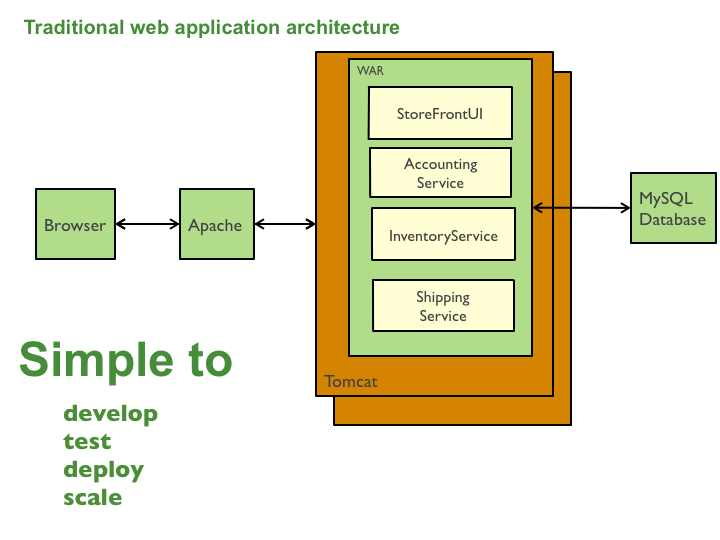
\includegraphics[width=0.9\linewidth]{images/TraditionalWebArchitecture}
		\caption{Traditionelle Webanwendungs Architektur}
		\label{fig:TraditionalWebArchitecture}
	\end{figure}

	\cite*{Richardson.2014} sieht jedoch auch eine Reihe von Nachteilen dieser Architektur, die mit zunehmender Größe der Anwendung und wachsender Teamgröße immer signifikanter werden.
	
	\begin{itemize}
	\item Die große monolithische Codebasis kann neue Entwickler schnell einschüchtern. Änderungen und Verständnis können schwierig sein und die Entwicklung verlangsamen. Durch fehlende Modulgrenzen geht im laufe der Zeit die Modularität verloren.
	\item Mit wachsender Größe er Codebasis werden die IDEs (Integrierte Entwicklungsumgeben) langsamer und bremsen die Produktivität
	\item Anwendungsstart wird zunehmend länger und hat einen großen Effekt auf die Produktivität der Entwickler und die Auslieferung. Wartezeit ist verschwendete Zeit.
	\item \textbf{Continuous deployment is difficult }
	\item Das Skalieren der Anwendung kann schwierig werden, da es nur in eine Dimension skalieren kann. Mit wachsenden Transaktionen kann das System durch zusätzlich Instanzen skaliert werden. Hingegen kann bei einem wachsenden Datenvolumen diese Architektur nicht gut skalieren. Jede Instanz greift auf alle Daten zurück und führt zu wenig effektivem Caching, höherem Speicherverbrauch sowie zusätzlichem I/O traffic. Außerdem können unterschiedliche Anwendungsbereiche verschiedene Anforderungen z.B. CPU haben, das skalieren von einzelnen Komponenten ist jedoch unmöglich.
	\item Die monolithische Architektur hat Grenzen wie die Entwicklung skalieren kann. Bei einer entsprechenden Anwendungsgröße werden Teams gebildet, die für spezielle Bereiche verantwortlich sind z.B. UI Team, Buchhaltungs Team etc.
	Die enge Verzahnung der einzelnen Bereiche erschwert jedoch die unabhängige Arbeit.
	\item Mit dem Beginn der Entwicklung muss sich auf eine Technologie und ggf. eine Version festgelegt werden, die es sehr schwer macht neue Technologien zu adaptieren. Eine inkrementelle Umstellung gestaltet sich als schwierig, wobei eine vollständige Ersetzung der aktuellen Technologie sehr kostenintensiv ist und das Problem im Kern nicht behebt.
	\end{itemize}
	\cite*[vgl. ][]{Richardson.2014}
	
	\subsection{Client/Server-Architekturmodell}
	Im Gegensatz zur monolitischen Architektur handelt es sich beim Client/Server Modell um ein verteiltes System.\\
	Das Client/Server-Architekturmodel ist ein Systemmodell, das aus einer Anzahl von zugehörigen Diensten und Servern besteht, sowie aus Clients, die diese Dienste nutzen und auf sie zugreifen. Das einfachste Modell ist dabei das zweischichtige Client/Server Modell, die zusammen ein komplettes System bilden mit unterschiedlichen Zuständigkeiten. \\
	Dabei lassen sich drei logische Hauptbestandteile unterschieden.
	
	\begin{figure}[h]
		\centering
		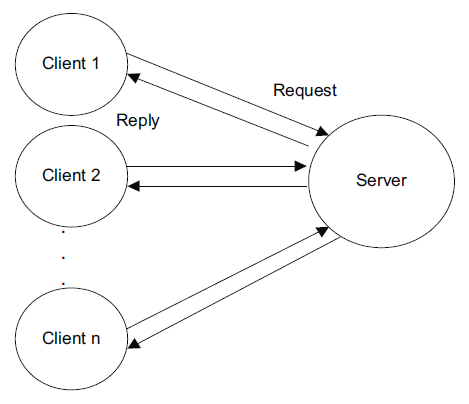
\includegraphics[width=0.7\linewidth]{images/Clients-und-Server}
		\caption{Client Server Model}
		\label{fig:client-server}
	\end{figure}
	
	\paragraph{Server}
	Der Server ist die zentrale Einheit der Architektur. Sie stellt Services und Daten anderen Einheiten zur Verfügung. Der Server muss nicht zwingend wissen, welche und wie viele Einheiten die von ihm zur Verfügung gestellten Dienste und Daten nutzen.
	
	\paragraph{Client}
	Clients können in beliebig großer Anzahl existieren. Sie nehmen die Daten oder Services, die vom Server bereitgestellt werden in Anspruch. Um mit den Diensten interagieren zu können, muss ein Client von der Existenz und dessen Adresse wissen. Der Client sendet eine Anfrage an den Server und bekommt ein Resultat zurück geliefert. \citet*[S. 302]{Sommerville.2007} unterscheidet folgende zwei Client-Modelle:
	\subsubsection{Thin-Client-Modell}
	Bei diesem Modell werden die gesamten Anwendungsprozesse und Datenhaltung auf dem Server erledigt. Der Client ist nur für die Darstellung verantwortlich. Daraus ergibt sich der Vorteil, dass sehr wenig Ressourcen für den Client benötigt werden und dieser sich auch auf kleinen Systemen (z.B. Terminals) implementieren lässt. Der Nachteil dieses Modelles liegt jedoch darin, dass so sämtliche Arbeit Serverseitig geleistet werden muss. Gerade bei Anwendungen mit großer Client Anzahl oder rechenintensiven Operationen kann so der Server schnell zur kritischen Komponente werden und das System vor Skalierungsprobleme stellen. Zusätzlich führt der Thin-Client zu einer erhöhten Netzwerkbelastung, da alle Daten vom Server zum Client transportiert werden müssen.
	
	\subsubsection{Fat-Client-Modell}
	Dieses Modell verlagert die Anwendungslogik vollständig oder in großen Teilen vom Server direkt in den Client. Dadurch kann der Server deutlich entlastet werden und die Rechenleistung des Client Rechners zusätzlich genutzt werden. Dies kann sich in speziellen Situationen allerdings auch als Nachteile erweisen, wenn die Client Computer die notwendige Rechenleistung nicht selbstständig bereitstellen könne. Der Server fungiert dabei nur noch als Daten Service und die Netzwerklast wird reduziert. Die Verlagerung der Anwendungslogik auf den Client bringt aber auch Nachteile mit sich. Müssen hier Änderungen vorgenommen werden, so müssen alle Clients auf die neue Version aktualisiert werden, was zu einem komplexen Systemmanagement führen kann. Der Aufwand dafür steigt mit zunehmender Zahl der Clients.
	
	\paragraph{Netzwerk (optional)}
	In der Literatur wird das Netzwerk häufig noch ein dritter Bestandteil aufgeführt, der jedoch nicht zwingend notwendig ist da prinzipiell Server und Client auf einem Computer ausgeführt werden können und so kein Netzwerk zur Kommunikation benötigen. Da dieses Modell aber in der Praxis nahezu ausschließlich als verteiltes System angewendet wird, ist in diesen Fällen das Netzwerk grundlegende Kommunikationsgrundlage.
	\\
	
	Generell hat das zweischichtige Client/Server Modell das Problem, dass die drei logischen Schichten auf zwei unterschiedlichen Computersystemen abgebildet werden müssen. \\
	
	\begin{figure}[h]
		\centering
		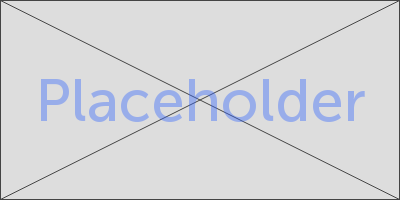
\includegraphics[width=0.7\linewidth]{images/placeholder}
		\caption{Logische drei Schichten}
		\label{fig:log3schichten}
	\end{figure}
	
	Als Alternativansatz hat sich dafür die dreischichtige Architektur Entwickelt. Sie stellt für jede logische Schicht ein separates Computersystem zur Verfügung. Die Vorteile liegen dabei in der besseren Skalierbarkeit, da jedes System individuell skaliert werden kann, geringere Netzwerklast im Vergleich zum Thin-Client-Modell und Anwendungsprozesse sind zentralisiert und lassen sich dort leichter anpassen und aktualisieren.
	

	\begin{figure}[h]
		\centering
		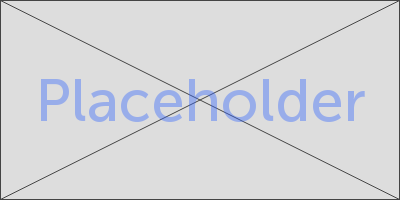
\includegraphics[width=0.7\linewidth]{images/placeholder}
		\caption{Drei schichtige Architektur}
		\label{fig:3-tier-architecture}
	\end{figure}


	Sommerville gibt in seinem Buch Software Engineering Beispiele, wann die Anwendung der jeweiligen Architektur sinnvoll ist.
	
	
	\begin{tabular}{|p{3.5cm}|p{12.5cm}|}
		\hline 
		Architektur & Anwendung \\ 
		\hline 
		Zweischichtige C/S-Architektur mit Thin-Clients & Anwendungen mit Legacy-Systemen, bei denen die Trennung von Anwendungsprozessen und Datenmanagement nicht praktikabel ist Rechenintensive Anwendungen wie zum Beispiel Compiler mit geringem oder keinem Datenmanagement -Datenintensive Anwendungen (Browser oder Abfragesysteme) mit wenig oder keinen Anwendungsprozessen \\
		\hline 
		Zweischichtige C/S-Architektur mit Fat-Clients & Anwendungen, bei denen die Prozesse durch Standardanwendungen (z.b. Microsoft Excel) auf dem Client verarbeitet werden Anwendungen mit rechenintensiver Datenverarbeitung (z.B. Datenvisualisierung) Anwendungen mit relativ stabiler Endbenutzerfunktionalität, die in einer Umgebung mit gut strukturiertem Systemmanagement angeordnet sind \\ 
		\hline 
		Drei- oder mehrschichtige C/S-Architektur & Anwendungen großen Umfangs mit Hunderten oder Tausenden von Clients Anwendungen, bei denen sowohl die Daten als auch die Anwendung selbst ständigen Veränderungen unterliegen Anwendungen, bei denen Daten aus vielfältigen Quellen verarbeitet werden \\ 
		\hline 
	\end{tabular} 
	
	
	
	\subsection{Dienstorientiert}

\section{System Kommunikation}
	\subsection{Represental State Transfer (REST)}
	REST wurde erstmals von 2000 Roy Thomas Fielding in seiner Dissertation beschrieben. Im Gegensatz zu bekannten Protokollen wie Simple Object Access Protokol (SOAP) oder XML-RPC handelt es sich bei REST um einen Architekturstil, wie Anwendungen basierend auf dem HTTP Protokoll miteinander kommunizieren können. Unterstützt eine Anwendung die REST-Stil, so bezeichnet man sie als RESTful.
	\cite[vgl.][]{Melzer.2010} \\
	REST basiert auf einem Konzept von Ressourcen, über die der Service Kenntnis hat. Der Server erstellt dabei verschiedene Darstellungen, wobei diese entkoppelt ist von der internen Speicherung.
	HTTP und HTTPS sind die primär benutzten Protokolle bei der Verwendung von REST. HTTP Caching Proxies, Load-Balancers und Monitoring Tools besitzen einen tiefe Unterstützung für HTTP von Haus aus.
	Den HTTP Verben GET, POST, PUT und DELETE lösen in RESTful Anwendungen spezielle Aktionen aus.
	\\
	
	\begin{tabular}{|p{3.5cm}|p{12.5cm}|}
	\hline 
	HTTP Verb & REST Aktion \\ 
	\hline 
	GET & Abfragen einer Ressource ohne Änderungen vorzunehmen \\ 
	\hline 
	POST & Erstellt eine neue Ressource. Der Link zur neuen Ressource wird zurück gegeben \\ 
	\hline 
	PUT & Eine Ressource wird angelegt. Wenn die Ressource bereits existiert, wird sie geändert. \\ 
	\hline 
	PATCH & Ein Teil der Ressource wird geändert \\ 
	\hline 
	DELETE & Löscht eine Ressource \\ 
	\hline 
	\end{tabular} 
	
	Der große Vorteil und der Grund für die schnelle Verbreitung von REST Architekturen liegt in der Einfachheit. Methoden für die Nutzung des HTTP Protokoll sind in allen modernen Programmiersprachen enthalten und können einfach genutzt werden. Das Ressourcen Konzept ist leicht anwendbar und bietet umfangreiche Möglichkeiten der eigenen Anpassung.
	
	Die Bandbreite der Möglichkeiten, die mit der REST Architektur umgesetzt werden können zeigt Leonard Richardson in seinem \textacutedbl Richardson Maturity Model\textgravedbl indem er vier REST Level beschreibt.

	\begin{figure}[h]
		\centering
		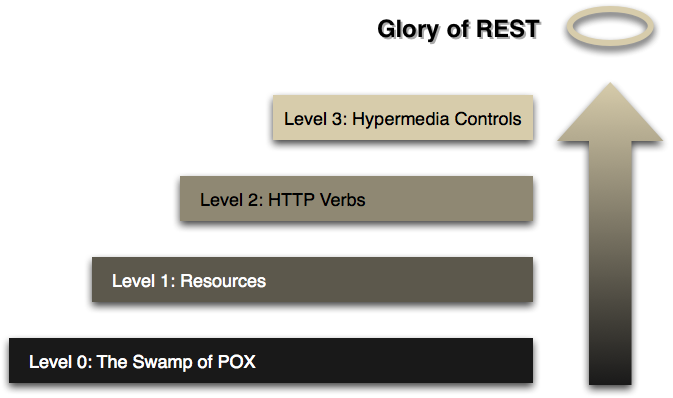
\includegraphics[width=0.7\linewidth]{images/Richardson_Maturity_Model}
		\caption{Richardson Maturity Model}
		\label{fig:Richardson_Maturity_Model}
	\end{figure}
	
	\cite[vgl.][]{Fowler.2010}
	\subsection{Enterprise Service Bus (ESB)}
	\subsection{Message Bus}

\section{Datenbanksysteme}
	\subsection{Relationale Datenbanken}
	\subsection{NoSQL Datenbanken}
	\subsection{Gegenüberstellung}
	
\section{Konzepte}
	\subsection{Singel Responisibility}
	\subsection{Domain Driven Design}
	\subsection{Data Consistency Primer}
	\subsection{Competiting Consumer Pattern}
	\subsection{Materialized View Pattern}
	\subsection{Queue-Based Lode Leveling Pattern}
	\subsection{Api Gateway Pattern}
